% Step 5 rewrite (2026-10-14): Results. Merges old Section 6 (discovery), the results of old Section 7 (controlled
% environments) and old Section 9 (decisions), ordered by RQ1-RQ3. New figures (Step 3, user-approved): fig_placebo,
% fig_maps, fig_logging_validity, fig_decisions; they replace fig_study1_discovery, fig_study2_maps,
% fig_study4_validity and fig_decision_referee. Moved to Appendix D: the validity table, the full map table with the
% placebo-calibrated and existence panels, the controlled-environment claims table, the full decision scorecard and the
% gate diagnosis. Every number is copied from the old sections and tables (journal ec32c22) or the figure modules'
% build-time assertions; the confounded-policy design-blind rates are from
% reviews/2026-10-13/briefs/N3_confounded_designblind.md (report.json V1_validity + V6_E4).
\section{Results}
\label{sec:results}

This section reports the results in the order of the research questions: the validity of the test
(Section~\ref{sec:res_validity}), the agreement with the ground truth (Section~\ref{sec:res_map}), the
role of the logging design in the controlled environments (Section~\ref{sec:study4}), and the conflict-mitigation
decisions (Section~\ref{sec:res_decision}).

\subsection{Validity}
\label{sec:res_validity}

PMRT made no declaration on the placebo logs of either dataset or on the null outcomes, and it met every validity
check of the protocol (Appendix~\ref{app:validity}). The baselines, in contrast, declared edges on placebo logs, up to
13 on the randomised logs and up to 29 on the confounded logs (Figure~\ref{fig:placebo}). Because the modes of the
randomised logs are independent of the network state, the declarations there arise from the baselines' thresholds
rather than from confounding. On the confounded logs, four of the seven baselines declared more placebo edges than on
the randomised logs, which is consistent with confounding adding to the threshold effect.

\begin{figure}[tbp]
\centering
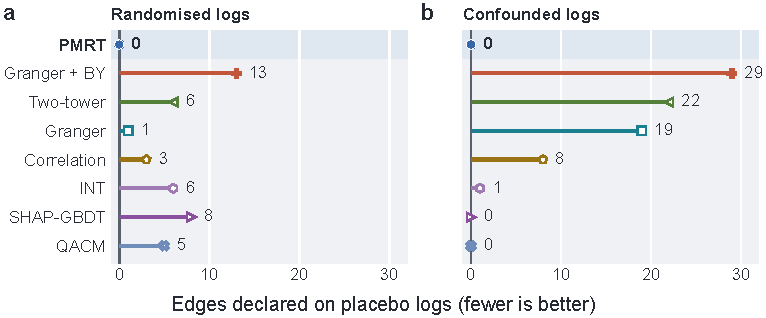
\includegraphics[width=\textwidth]{figures/fig_placebo.pdf}
\caption{Edges declared on placebo logs.}
\label{fig:placebo}
\end{figure}

The validity checks also showed three departures from exactly nominal behaviour, none of which led to a declaration.
On the randomised placebo logs, 7 of the 60 p-values were at or below 0.05 where 3 were expected; the binomial tail
probability of 0.03 remained above the protocol limit of 0.01. The null-outcome check used 999 redraws, with which a
declaration was unattainable, so it was repeated with 9\,999 redraws, which produced declarations in 2 of 590
variants, within the limit of 7.5~\%. Finally, the hypotheses that the ground truth labels
null are small effects rather than sharp nulls. Over all 21, the rate of p-values at or below 0.05 was 0.15, about
three times nominal, which reflects real effects below the materiality threshold. Over the 12 whose knockout interval
also contains zero it was 0.075, with an interval reaching 0.16, so that an excess cannot be excluded there either.

\subsection{Agreement with the ground truth}
\label{sec:res_map}
\label{sec:study1}
\label{sec:study2}
\label{sec:map_claims}

PMRT's maps agreed closely with the knockout ground truth (Figure~\ref{fig:maps}). On the randomised logs it declared 28
edges, with a precision of 0.92, a recall of 0.79 and no wrong sign. On the confounded logs, where the incumbent's
state-dependent propensities were logged, it declared 22 edges, with a precision of 0.86, a recall of 0.62 and again no
wrong sign (Table~\ref{tab:maps}). It declared the edge from pico sleep to neighbour protected-slice violations, on which the
scenario's conflict rests, and the other three edges of the conflict chain, each with the ground-truth sign, on both
kinds of log and in every larger subsample of the randomised logs. Of the ten true neighbour-relation edges it declared nine,
missing only the edge from pico sleep to neighbour RLFs. The baselines either declared far fewer true edges or reached
a higher recall only with wrong signs and false edges. Granger~+~BY, the strongest of them, reached a recall of 0.55 with six
wrong signs on each kind of log and a precision of 0.59 and 0.54. Calibrating the baselines' thresholds on the placebo
logs themselves removed their placebo declarations, but only in-sample and at the cost of recall, which fell to at
most 0.21 (Appendix~\ref{app:maps_full}).

\begin{figure}[tbp]
\centering
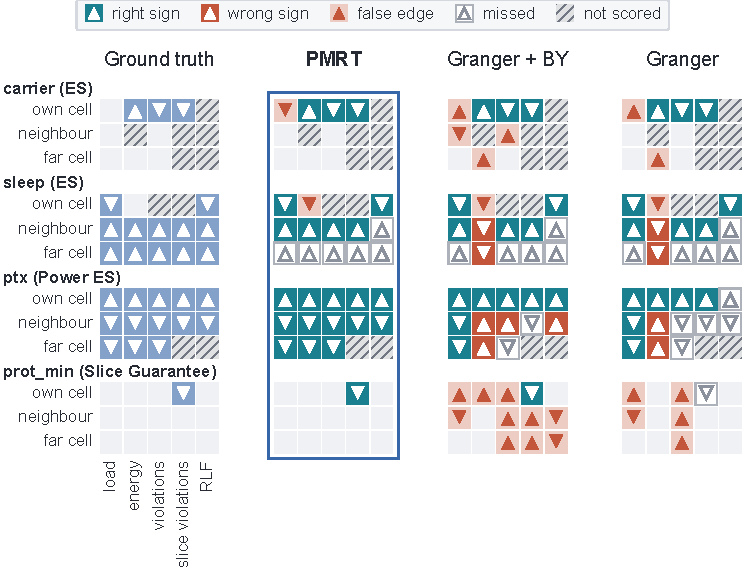
\includegraphics[width=\textwidth]{figures/fig_maps.pdf}
\caption{Causal maps learned from randomised logs.}
\label{fig:maps}
\end{figure}

\begin{table}[tbp]
\caption{Map quality on randomised / confounded logs.}
\label{tab:maps}
% Precision = (R + W) / (R + W + N) and recall = right-sign recall over the 29 true hypotheses, from the old
% tab:maps (journal ec32c22), DEV-tuned thresholds; placebo edges as in fig_placebo.
\setlength{\tabcolsep}{4pt}
\begin{tabular*}{\textwidth}{@{\extracolsep{\fill}}l c c c c@{}}
\toprule
Method & Precision & Recall & Wrong signs & Placebo edges \\
\midrule
PMRT         & 0.92 / 0.86 & 0.79 / 0.62 & 0 / 0 & 0 / 0 \\
Granger + BY & 0.59 / 0.54 & 0.55 / 0.55 & 6 / 6 & 13 / 29 \\
Granger      & 0.69 / 0.60 & 0.48 / 0.41 & 4 / 6 & 1 / 19 \\
QACM         & 0.89 / 0.83 & 0.28 / 0.17 & 0 / 0 & 5 / 0 \\
INT          & 0.88 / 0.80 & 0.24 / 0.14 & 0 / 0 & 6 / 1 \\
Correlation  & 0.86 / 0.80 & 0.17 / 0.21 & 1 / 2 & 3 / 8 \\
Two-tower    & 1.00 / 0.63 & 0.17 / 0.17 & 1 / 0 & 6 / 22 \\
SHAP-GBDT    & 1.00 / 0.50 & 0.03 / 0.03 & 0 / 0 & 2 / 2 \\
\bottomrule
\end{tabular*}
\end{table}

One protocol criterion on the randomised logs was not met. It required PMRT's F1 score on the neighbour-relation edges
to equal or exceed that of each of three baselines on most small subsamples. Against Granger~+~BY the condition held on only 2
of the 10 smallest subsamples, although it held on 4 of the 5 larger ones, so that the discovery verdict on these logs
was partial (Online Resource~1, Section~S1.1). The F1 ranges of the two methods overlapped on the smallest subsamples, and
the criterion did not account for the 13 placebo edges of Granger~+~BY. Discovery on the confounded logs met every
criterion.

Precision depends on how the ground truth is defined. Against the materiality threshold used throughout, it was 0.92
and 0.86;
with the threshold halved it rose to 1.00 on both kinds of log, and with it doubled it fell to 0.59 and 0.73. The fall
reflects real effects below the doubled threshold rather than wrong declarations. Under an existence rule, which
counts any effect whose knockout interval excludes zero, 26 of PMRT's 28 declarations on the randomised logs and all
22 on the confounded logs were real effects with the declared sign (Appendix~\ref{app:x11}). PMRT made no wrong-sign
declaration under any ground-truth variant, and its neighbour and far declarations were almost all labelled true, 12 of
13 on the randomised logs and all 7 on the confounded logs. Under the doubled threshold, however, the ranking of
methods is not preserved: the small maps of INT, QACM and two-tower kept precisions of 0.88, 0.80 and 0.83 on the
randomised logs, above PMRT's 0.59, although at recalls of 0.35, 0.40 and 0.25 against its 0.80.

\subsection{Role of the logging design}
\label{sec:study4}
\label{sec:study4_results}
\label{sec:study4_verdicts}

The controlled environments confirm that validity derives from the logging design. Tests that ignored the design
were close to their nominal rate under independent logging but lost it once actions followed a dithered setpoint, with
null-edge rates of 0.33 to 0.94, whereas the design-based and design-adjusted tests remained near 0.05 under every
logging design (Figure~\ref{fig:logging_validity}). All four claims fixed in the protocol were supported
(Online Resource~1, Section~S4.1), with two exceptions. Design-adjusted RCoT was invalid even with the design covariates,
and PMRT-Lin, the secondary linear variant, exceeded its allowance of invalid conditions under the confounded policy,
although its pooled rates were valid and a re-run on fresh datasets gave rates consistent with chance.

\begin{figure}[tbp]
\centering
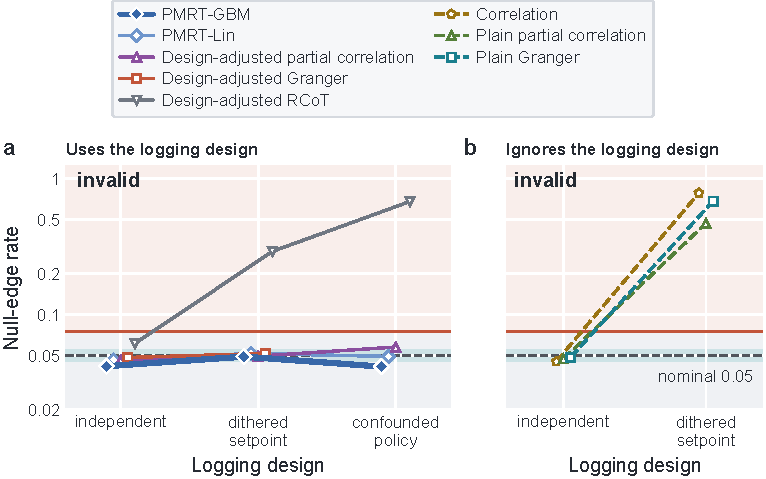
\includegraphics[width=\textwidth]{figures/fig_logging_validity.pdf}
\caption{Null-edge rate by logging design.}
\label{fig:logging_validity}
\end{figure}

The latent-confounding environment illustrates the mechanism most directly, because there the associational sign is
reversed at large confounding strength. Under the logged confounded policy, the null-edge rate of correlation was 1.00 whenever the
confounding was present, while that of PMRT-GBM stayed between 0.02 and 0.06 in every condition. Validity under this
policy is not specific to PMRT: design-adjusted partial correlation also stayed valid. The protocol did not score the
design-blind tests under the confounded policy; descriptively, correlation and plain RCoT were far above nominal there,
at 0.77 and 0.23, whereas plain partial correlation stayed near nominal, at 0.056, most likely because the confounder
was among its covariates. A post hoc variation of the dither width and of the number of setpoints left correlation
invalid and the two PMRT methods between 0.042 and 0.054. Under unlogged confounding, the negative control, the real
actions have no logged design, and on the placebo edge the rates of the design-based tests were never invalid.

The same environments also show the limits of a placebo check. With its threshold calibrated on the placebo column,
the discovery stage of CDD O-RAN passed that check but exceeded the nominal null-edge rate in 9 of 30 conditions. A
pipeline that declares placebo edges, as every baseline did on the randomised logs, is thus shown to be invalid, whereas
a pipeline that passes the check may still be invalid. The check is therefore a necessary condition for validity, but
not a sufficient one.

\subsection{Conflict mitigation}
\label{sec:res_decision}
\label{sec:res_referee}
\label{sec:study3}

Without the gate, the PMRT referee reached the highest recovery of any referee, $R = 0.47$, but breached the RLF guard
and was therefore ineligible (Figure~\ref{fig:decisions}, Table~\ref{tab:decision_e2e}). Its RLF ratio was 1.31
(90~\% confidence interval, CI, 1.10 to 1.56), against the limit of 1.10. The breach came from rejected transmit-power requests.
PMRT's map from the confounded logs lacked the edge from the transmit-power offset to neighbour RLFs, which the ground
truth labels true; the oracle map holds this edge, so its guard-conflict rule accepts the next power-up unit after each
rejected one. Over all seeds, PMRT's referee rejected 8\,674 power-up units against the oracle map's 2\,370, while
their sleep rejections were similar. PMRT's primary statistic had missed this edge ($p = 0.49$); an unfiltered
statistic, examined after the fact and not used, would have detected it.

\begin{figure}[tbp]
\centering
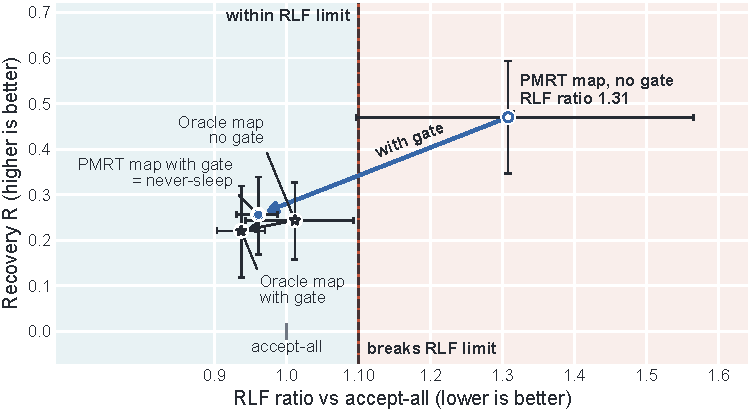
\includegraphics[width=\textwidth]{figures/fig_decisions.pdf}
\caption{Recovery against RLF ratio, without and with the gate.}
\label{fig:decisions}
\end{figure}

\begin{table}[tbp]
\caption{Decision outcomes.}
\label{tab:decision_e2e}
% From the old full scorecard (now Table tab:decision_full in Appendix D); 90 % paired seed-bootstrap CIs.
\setlength{\tabcolsep}{4pt}
\begin{tabular*}{\textwidth}{@{\extracolsep{\fill}}l c c c c@{}}
\toprule
Arm & $R$ & $R$ minus never-sleep [90~\% CI] & RLF ratio & Eligible \\
\midrule
\multicolumn{5}{@{}l}{\textit{Without the gate}} \\
\quad Accept-all & 0.00 & $-0.22$ [$-0.30$, $-0.14$] & 1.00 & yes \\
\quad Never-sleep & 0.22 & -- & 0.99 & yes \\
\quad PMRT map & 0.47 & $+0.25$ [$0.14$, $0.36$] & 1.31 & no \\
\quad Oracle map & 0.24 & $+0.02$ [$-0.04$, $0.09$] & 1.01 & yes \\
\midrule
\multicolumn{5}{@{}l}{\textit{With the gate}} \\
\quad Accept-all & 0.00 & $-0.26$ [$-0.34$, $-0.17$] & 1.00 & yes \\
\quad Never-sleep & 0.26 & -- & 0.96 & yes \\
\quad PMRT map & 0.26 & $0.00$ [$0.00$, $0.00$] & 0.96 & yes \\
\quad Oracle map & 0.22 & $-0.04$ [$-0.10$, $0.03$] & 0.94 & yes \\
\bottomrule
\end{tabular*}
\end{table}

With the gate, the PMRT referee met every guard but made the same decisions as the never-sleep rule: on every seed its
outcomes were identical to those of never-sleep, so its gain in recovery over that rule, the primary criterion, was
zero. The protocol had anticipated this tie and kept the criterion unchanged, since dropping it would have changed a
criterion in view of an expected result. No gated referee improved on never-sleep; the oracle map differed from it by $-0.04$ (90~\% CI $-0.10$ to
$0.03$). The gated runs used fresh seeds, and on them the ungated PMRT referee, run as a descriptive arm, no longer
outperformed never-sleep, differing by $-0.06$ at an RLF ratio of 1.05. Pooled over both seed sets, its gain was small, 0.10 with an
interval that barely excludes zero, and its RLF ratio of 1.18 still breached the guard. The two seed sets did not
differ at the network level, but the referee's per-seed gain was heavy-tailed and its mean differed between them. The
rule stated in advance did not cover this case, so the non-replication was attributed after the results had been seen
to seed-level heterogeneity of an adaptive referee, and the pooled estimate is taken as the best estimate
(Appendix~\ref{app:x15}).
Referees using the associational maps, finally, raised protected-slice violations to 4.5 to 5.4 times the accept-all
level, because they rejected Slice Guarantee's protected-share requests; several stayed eligible, since the protected
slice has no guard of its own (Appendix~\ref{app:decision_full}).

\label{sec:disc_decision}
The gate accounts for the absence of a gain from a valid map. Of the request classes that the PMRT map allows the
referee to reject, the gate certified only putting picos to sleep. It withheld the transmit-power-up rejections because their two
unresolved guard edges, to neighbour RLFs and far service violations, are true in the ground truth, with point
estimates of harm above their tolerances, so that more logging would not have certified them (Appendix~\ref{app:gate}).
The oracle map certifies this class only because it declares both edges, and its gated referee gained over never-sleep
only in energy retention, 1.29 against 1.15. Rejecting more requests does not compensate for this: a referee that rejected
requests at random, at the rate of the ungated referee, had negative recovery. In this scenario, therefore, the guards
and the objective, rather than the map, limited the benefit of safe decisions.
